\documentclass[10pt]{beamer}
%\documentclass[10pt, handout]{beamer}
\setbeameroption{show notes}

%\documentclass[10pt, a4paper]{article}
%\usepackage{beamerarticle}




\mode<article>{
	
	\usepackage{hyperref}
	
}
\mode<presentation>{
	
	\usetheme{Antibes}
	\usefonttheme{professionalfonts} 
	\usefonttheme{serif} % default family is serif
	
	%\usecolortheme{spruce} %зеленая, плохой цвет в заголовках 
	%\usecolortheme{albatross} %синяя, пхоло виден черный цвет
	
}

\newcommand{\MP}[1]{\mode<presentation>{#1} }
\newcommand{\MA}[1]{\mode<article>{#1} }

\newcommand{\ABS}[1]{\left| #1 \right|}
%\newcommand{\ABS}[1]{\mid #1 \mid}

\newcommand{\HREF}[2]{{\color{blue}\underline{\href{#1}{#2}}}}

\setbeamertemplate{caption}[numbered]


%\usepackage[T2A]{fontenc}
%\usepackage[utf8]{inputenc}
%\usepackage[russian]{babel}
%\usepackage{amsmath} %математические формулы



\usepackage{ifthen}

\usepackage{tikz}
\usetikzlibrary{arrows.meta}
\usetikzlibrary{calc}
\usetikzlibrary{decorations}
\usetikzlibrary{decorations.pathreplacing}
\newcommand{\rememb}[1]{\tikz[remember picture,baseline=-0.5ex]{\draw node[inner sep=0pt, outer sep=0pt] (#1){\strut};}}



\usepackage{fp}
\usepackage{tikz-3dplot}
\usepackage{environ}
\usepackage{animate}





\usepackage{xcolor}
%\usepackage[left=20mm,right=20mm,top=20mm,bottom=20mm,a4paper]{geometry} %поля

\usepackage{amsmath} %математические формулы
%\usepackage{amsfonts} %математические шрифты


\usepackage[e]{esvect}  %Красивая стрелочка вектора
%\let\oldvv\vv
\newcommand{\VV}[1]{\vv{#1\mathstrut}}



\usepackage{graphicx} %работа с каритнками


%\usepackage{multimedia}
%\usepackage{movie15}

%Для XeLatex/+
\usepackage{polyglossia}
\setdefaultlanguage{russian}
\setotherlanguage{english}
%\setkeys{russian}{babelshorthands=true} 


\usepackage{fontspec}

\setmainfont{Times New Roman} [Script=Cyrillic, Mapping=tex-text,]
\setsansfont{Arial} [Script=Cyrillic, Mapping=tex-text,]
%\setmonofont{Courier New} [Script=Cyrillic, Mapping=tex-text,]
\newfontfamily{\cyrillicfonttt}{Courier New}


%\usepackage{unicode-math}
%\setmathfont{TeX Gyre Termes Math}

%\setmainfont{CMU Serif}[Script=Cyrillic, Mapping=tex-text,]
%\setsansfont{CMU Sans Serif}[Script=Cyrillic, Mapping=tex-text,]
%\setmonofont{CMU Typewriter Text}[Script=Cyrillic, Mapping=tex-text,]


%-----------------


%\usepackage{caption}
%\DeclareCaptionLabelSeparator{dot}{~---~}            %Разделитель номер рисунка
%\captionsetup[figure]{justification=centering,labelsep=dot, format=plain}                        %Подпись рис. центр
%\captionsetup[table]{justification=raggedleft,labelsep=dot, format=plain, singlelinecheck=false} %Подпись табл. слева
%\captionsetup[lstlisting]{justification=raggedleft,labelsep=dot, format=plain, singlelinecheck=false}                     %Подпись рис. центр

\usepackage{indentfirst} %отступ первой строки


\usepackage[svgnames]{xcolor}


\usepackage{hyperref}

%\usepackage{showframe}


%\usepackage{tikz}

%\usepackage[hidelinks]{hyperref}%ссылки внутри документа \ref


\setlength\abovecaptionskip{-2pt}
%\setlength\belowcaptionskip{-14pt}

\setbeamerfont{caption}{size=\scriptsize}


\def\sectionname{Раздел}
\def\subsectionname{Подраздел}


\newcommand{\TC}[3]
{
	
	
	\begin{columns}
		\begin{column}{#1\textwidth}
			#2
		\end{column}
		\begin{column}{\fpeval{1-#1}\textwidth}
			#3
		\end{column}
	\end{columns}
}

\newcommand{\TCT}[3]
{
	
	\begin{columns}[T]
		\begin{column}{#1\textwidth}
			#2
		\end{column}
		\begin{column}{\fpeval{1-#1}\textwidth}
			#3
		\end{column}
	\end{columns}
}


\newcommand{\FRAME}[2]{
	\begin{frame}
		\frametitle{#1}
		#2
	\end{frame}
}

\newcommand{\FIG}[3]
{
	\begin{figure}
		\centering
		\includegraphics[width=#3]{#1}
		\caption{#2}
	\end{figure}
}

\newcommand{\vect}[1]{\overrightarrow{#1}}


\usepackage{qrcode}

\newcommand{\LECADDR}{https://clck.ru/3D3Efj}


\usepackage{newfile}

\edef\LectionNumber{0}
\edef\LectionTheme{0}

\let\oldsection\section
\let\oldsubsection\subsection


\AtBeginDocument
{
	\newoutputstream{CONTENT}
	\openoutputfile{\LectionNumber .gvr}{CONTENT}
	
	\expandafter\addtostream{CONTENT}{\noindent\textbf{\Large Лекция \LectionNumber~---~\LectionTheme}\unexpanded{\setcounter{SEC}{0}}\par}
}

\renewcommand{\section}[1]{
	\oldsection{#1}
	\expandafter\addtostream{CONTENT}{\noindent\hspace{2ex}\unexpanded{\hbox{\large\stepcounter{SEC}\theSEC ~ #1}}\par}
}

\renewcommand{\subsection}[1]{
	\oldsubsection{#1}
	\expandafter\addtostream{CONTENT}{\noindent\hspace{6ex}\unexpanded{\stepcounter{SUB}\theSUB ~ #1}\par}
}


%\renewcommand{\section}[1]{\MMM{#1}}

%\edef\subsection#1
{
	%\noexpand\subsection{#1}
	%
}


\newfontfamily\dnifamily[Scale = 0.795]{DniFont.TTF}

\newcommand{\dni}[1]{%
	{\dnifamily%
		\ifthenelse{#1=0}{0}{}%
		\ifthenelse{#1=1}{1}{}%
		\ifthenelse{#1=2}{2}{}%
		\ifthenelse{#1=3}{3}{}%
		\ifthenelse{#1=4}{4}{}%
		\ifthenelse{#1=5}{5}{}%
		\ifthenelse{#1=6}{6}{}%
		\ifthenelse{#1=7}{7}{}%
		\ifthenelse{#1=8}{8}{}%
		\ifthenelse{#1=9}{9}{}%
		\ifthenelse{#1=10}{)}{}%
		\ifthenelse{#1=11}{!}{}%
		\ifthenelse{#1=12}{@}{}%
		\ifthenelse{#1=13}{\#}{}%
		\ifthenelse{#1=14}{\$}{}%
		\ifthenelse{#1=15}{\%}{}%
		\ifthenelse{#1=16}{\^{}}{}%
		\ifthenelse{#1=17}{\&}{}%
		\ifthenelse{#1=18}{*}{}%
		\ifthenelse{#1=19}{(}{}%
		\ifthenelse{#1=20}{[}{}%
		\ifthenelse{#1=21}{]}{}%
		\ifthenelse{#1=22}{\textbackslash{}}{}%
		\ifthenelse{#1=23}{\{}{}%
		\ifthenelse{#1=24}{\}}{}%
		\ifthenelse{#1=25}{|}{}}%
}%

\newcommand{\toDni}[1]{%	
	\ifthenelse{#1=0}{}{%
		 \ifthenelse{#1=25}{%
		 	\expandafter\dni{#1}}{%
		 	\expandafter\toDni{\fpeval{floor(#1/25)}}%
		 \expandafter\dni{\fpeval{(#1/25 - floor(#1/25))/0.04}}}}%
}%



\newcommand{\Strut}{{\Large\strut}}

\newcommand\scb[1]{\left( #1 \right)}

\newcommand{\LINK}[2]{%
	\qrcode[height=1cm]{#1}\  \HREF{#1}{\parbox{0.8\textwidth}{#2}} \\[0.5em]
}

\NewDocumentCommand{\lecdni}{}{\toDni{\LectionNumber}}
\author{Гаврилов Андрей Геннадьевич}
\newcommand{\regals}{кандидат технических наук, доцент}
\institute{Кафедра Информационных технологий и вычислительных систем \\МГТУ~<<СТАНКИН>>}
\lecture{История компьютерной графики}{kghistory}\subtitle{Компьютерная графика}


\makeatletter
\newcommand*{\overlaynumber}{\number\beamer@slideinframe}
\makeatother



\usepackage{cprotect}

\newcommand{\QRFRAME}{%
    \begin{frame}[plain, noframenumbering]    	
	
	\centering
	Трансляция презентации (во время очных лекций)    
	
	~
	
	{\Large \ttfamily  https://clck.ru/3D3Efj  }
	
	~
	
	\tikz\node[inner sep=0pt,rounded corners=5mm, clip]{\qrcode[height=0.45\textwidth]{\LECADDR}}; 
	
	~	
	{\small
	При просмотре презентации в PDF для отображения анимаций на слайдах необходимо использовать Acrobat Reader, KDE Okular, PDF-XChange, Foxit Reader, браузер Firefox. Для браузеров на движке Chrome (Edge, Яндекс, Opera,~\dots) необходимо использовать \HREF{https://chromewebstore.google.com/detail/pdf-viewer/oemmndcbldboiebfnladdacbdfmadadm?hl=ru&utm_source=ext_sidebar}{PDF.js} c опцией <<Enable active content (JavaScript) in PDFs>>. }
	
	\end{frame}%
}

\newcommand{\IG}[2][1]{\includegraphics[width=#1\textwidth]{#2}}



\graphicspath{{Images/}{Images/\jobname/}}

\date{\today}



\renewcommand{\LectionNumber}{7}
\renewcommand{\LectionTheme}{Вращение пространства}
\title{Лекция \lecdni \\ \LectionTheme}
\subtitle{Компьютерная графика}



%\usepackage{standalone}

\setbeamersize
{
	text margin left=0.5cm,
	text margin right=0.5cm
}

\usepackage{comment}


%	\transduration{2}
%   \transfade

 \begin{document}
 		 
	\makeatletter
\defbeamertemplate*{title page}{my theme}
{
	
	\hfill
	
	\begin{beamercolorbox}[wd=.9\paperwidth,center,]{title}%
		
	\end{beamercolorbox}%	
	
	\vbox to 1em {}
	
	\begin{beamercolorbox}[wd=.9\paperwidth,center,]{title}%
		\usebeamerfont{subtitle}%
		\hfill
		
		\insertsubtitle
		
		\usebeamerfont{title}%
		\inserttitle{} \\[0.5em]
		
		
		
	\end{beamercolorbox}%	
	\hfill\hfill
	
	\begin{beamercolorbox}[wd=.9\paperwidth,center,]{}%
		\usebeamerfont{author}%
		\hfill \\[0.5em]
		\insertauthor{} \\[0.5em]
		\regals
		    
		\vbox to 1em{}
		\usebeamerfont{institute}%
		\insertinstitute {}
		
		\vbox to 1em{}			
		{\; }\insertshortdate{}
		
	\end{beamercolorbox}%	
	\hfill\hfill
	
	\vbox to 5em{}
	
	
}
\defbeamertemplate*{footline}{my theme}{
	\leavevmode%
	\hbox{%
		\begin{beamercolorbox}[wd=.25\paperwidth,ht=3.25ex,dp=0ex,center,sep=1pt]{author in head/foot}%
			\usebeamerfont{author in head/foot}%
			\insertauthor 
			\beamer@ifempty{\insertshortinstitute}{}
		\end{beamercolorbox}%
		\begin{beamercolorbox}[wd=.65\paperwidth,ht=3.25ex,dp=0ex,center,sep=1pt]{title in head/foot}%
			\usebeamerfont{title in head/foot}\insertshortinstitute
		\end{beamercolorbox}%
		\begin{beamercolorbox}[wd=.1\paperwidth,ht=3.25ex,dp=0ex,center, sep=0.5pt]{date in head/foot}%
			\usebeamerfont{date in head/foot}
			\footnotesize \expandafter\toDni{\insertframenumber} / \expandafter\toDni{\inserttotalframenumber}
	\end{beamercolorbox}}%
}



\makeatother






%float page top aligment
\makeatletter
\setlength{\@fptop}{0pt}
\setlength{\@fpbot}{0pt plus 1fil}
\makeatother

\newcommand \abs[1] {\left| #1 \right|}

\everymath{\displaystyle}

    
    \QRFRAME	
	

	\frame{\maketitle}

	
	\begin{frame}{План лекции}
		\tableofcontents
	\end{frame}
	
	\section{Вращения в $\mathbb R^2$}
	
	\begin{frame}{Пространство вращения}
		
		\TC{0.35}
		{
			\includegraphics[page=1]{2drotationspace.pdf}
		}
		{
			\only<2>{\includegraphics[page=2,scale=0.9]{2drotationspace.pdf}}%	
			\only<3>{\includegraphics[page=3]{2drotationspace.pdf}}%	
		}
		
	\end{frame}
	

		
	
	
	\begin{frame}{Числа}
		\centering 
		
		\foreach \t in {1,...,4}{%
			\only<\t>%
			{%
				\includegraphics[page=\t]{digit_axis.pdf}%
			}%
		}		
		
		\TC{0.6}
		{
			\foreach \t in {1,...,4}{%
				\only<\t>%
				{%
					\includegraphics[page=\t]{digit_circles.pdf}%
				}%
			}
		}
		{
			\begin{enumerate}
				\item <+-> $3+x=6$
				\item <+-> $9+x=6$
				\item <+-> $3x=7$
				\item <+-> $x^2=5$
			\end{enumerate}		
		
		}		
	\end{frame}
	
	


	
	\begin{frame}{Компл\'ексные числа}
		
		\TC{0.5}
		{
			\only<1-2>{\includegraphics[page=1]{enter_complex.pdf}}%
			\only<3>{\includegraphics[page=2]{enter_complex.pdf}}%
			\only<4>{\includegraphics[page=3]{enter_complex.pdf}}%
			\only<5-6>{\includegraphics[page=4]{enter_complex.pdf}}%
			\only<7->{\includegraphics[page=6]{enter_complex.pdf}}%
			
			\onslide<1->{$x^2=-1$}%
			\onslide<2->{. Введём число $i: i^2=-1$}%
			
			\onslide<2->{$x=\sqrt{-1}, x=\pm i$}%
			
			~
			
			\onslide<4->{\fbox{$z=a+bi$}, $a,b \in \mathbb{R}$}%
			
			\onslide<4->{$a$ --- действительная часть}%
			
			\onslide<4->{$b$ ---  мнимая часть}%
		}{
			\onslide<5->{$\|z\|=a^2+b^2$ --- норма к.\,ч.}%
			
			\onslide<5->{$|z|=r=\sqrt{\|z\|}$ --- модуль к.\,ч.}%
			
			\onslide<5->{$\varphi = \arg(z)=\arctan (b/a)$ --- аргумент к.\,ч.}%
			
			~
			
			\onslide<6->{$z=r(\cos \varphi +i\sin \varphi)$ --- тригоном. форма}%
			
			\onslide<6->{$z=re^{i\varphi}$ --- показательная форма}%
			
			~
			
			\onslide<7->{$\bar z =a-bi=re^{-i\varphi}$ --- сопряжённое к.\,ч.}%
			
			\onslide<7->{$-z=(-1)z=-a-bi=-re^{-i\varphi}$}%
			
			~
			
			\onslide<8->{$(a+bi)+(\alpha+\beta i) = (a+\alpha)+(b+\beta)i$}%
			
			\onslide<8->{$(a+bi)(\alpha+\beta i) = (a\alpha-b\beta)+(a\beta+b\alpha)i$}%
			
			\onslide<8->{$re^{i\varphi}\cdot pe^{i\psi}=rpe^{i(\varphi+\psi)}$}%
			
			~
			
			\onslide<9->{$z\bar z = a^2+b^2 = \|z\|$}%
			
			
		}
		
		
	\end{frame}
	

	
	\begin{frame}{Частные случаи}
		\TC{0.4}
		{
			\includegraphics[page=2]{digit_circles2.pdf}
		}
		{
				\onslide<1->{%
				Если $z_1=a+bi:b=0 \Leftrightarrow z\in \mathbb{R}$
				
				$\forall z \in \mathbb R ( \ {-z} = \bar z )$
				}
				
				~
				
				\onslide<2>{%
				Если $z_2=a+bi:a=0 \Leftrightarrow z\in \mathbb{I}$
				}
				
				~
				
				\only<1>{\includegraphics[page=1]{enter_complex2.pdf}}%
				\only<2>{\includegraphics[page=2]{enter_complex2.pdf}}%
		}
	\end{frame}
	
		
	\begin{frame}{Вращение плоскости}
		\TC{0.4}
		{
			\animategraphics[autoplay,loop, nomouse]{15}{Images/\jobname/rotor}{0}{358}
		}
		{
			\textbf{Задача.} Повернуть радиус-вектор $z$ на угол $\psi$.
			
			~\pause
			
			$\vv z = (a,b) \Rightarrow z=(a+bi) \Rightarrow z=re^{i\varphi}$
			
			~\pause
			
			Делаем поворот на $\psi$: 
			$re^{i\varphi}\cdot e^{i\psi} = re^{i(\varphi+\psi)} \Rightarrow {}$
			${}\Rightarrow z=a'+b'i \Rightarrow \vv {z'} = (a',b') $.
			
			~\pause
			
			$R(\psi) \rightarrow e^{i\psi}$
			
			$R(\varphi)\circ \ldots \circ R(\psi) = e^{i\varphi}\ldots e^{i\psi}$
			
			~
			
			$R(\varphi)\circ R(\psi)=R(\psi)\circ R(\varphi)$
			
			
			
		}
		
	\end{frame}
	
	\section{Вращения в $\mathbb R^3$}
	
	
	\begin{frame}{А как вращать $\mathbb R^3$? Матрицы!! (нет)}
		\footnotesize
		\TC{0.5}
		{
			\begin{block}{Матрица поворота вокруг $OX$}
				\centering 
				$ \mathbf R_x(\alpha)
				=
				\begin{pmatrix}
					1&0&0&0\\
					0&\cos\alpha&-\sin\alpha&0\\
					0&\sin\alpha&\cos\alpha&0\\
					0&0&0&1				 	
				\end{pmatrix}
				$				
			\end{block}
		}
		{
			\begin{block}{Матрица поворота вокруг $OY$}
				\centering 
				$ \mathbf R_y(\beta)
				=
				\begin{pmatrix}
					\cos\beta&0&\sin\beta&0\\
					0&1&0&0\\
					-\sin\beta&0&\cos\beta &0\\
					0&0&0&1				 	
				\end{pmatrix}
				$				
			\end{block}
		}
		
		\begin{columns}
			\begin{column}{0.25\textwidth}
				~
			\end{column}
			\begin{column}{0.5\textwidth}
				\begin{block}{Матрица поворота вокруг $OZ$}
					\centering 
					$ \mathbf R_z(\gamma)
					=
					\begin{pmatrix}
						\cos\gamma&-\sin\gamma&0&0\\
						\sin\gamma&\cos\gamma&0&0\\
						0&0&1&0 \\
						0&0&0&1	\\			 	
					\end{pmatrix}
					$				
				\end{block}
			\end{column}
			\begin{column}{0.25\textwidth}
				~
			\end{column}
		\end{columns}
		
		\begin{block}{Матрица поворота вокруг произвольной оси $\vv v$, $|\vv v| = 1$}
			\centering\scriptsize$
			\mathbf{R}(\vv v, \theta) = 
			\begin{pmatrix}
				\cos \theta + (1 - \cos \theta) x^2
				& (1 - \cos \theta) x y - (\sin \theta) z 
				& (1 - \cos \theta) x z + (\sin \theta) y  
				& 0\\
				(1 - \cos \theta) y x + (\sin \theta) z 
				& \cos \theta + (1 - \cos \theta) y^2
				& (1 - \cos \theta) y z - (\sin \theta) x
				& 0\\
				(1 - \cos \theta) z x - (\sin \theta) y
				& (1 - \cos \theta) z y + (\sin \theta) x
				& \cos \theta + (1 - \cos \theta) z^2 
				& 0 \\
				0 & 0 & 0 & 1
			\end{pmatrix}
			$
		\end{block}
	\end{frame}
	
	
	\begin{frame} {Пространство вращения}
		
		\centering
		
		\parbox[c]{0.4\textwidth}{%
			\only<1>{\includegraphics[page=2]{xyrotationaxis.pdf}}%
			\only<2>{\includegraphics[page=4]{xyrotationaxis.pdf}}%
			\only<3>{\includegraphics[page=6]{xyrotationaxis.pdf}}%
			\only<4>{\includegraphics[page=8]{xyrotationaxis.pdf}}%
			\only<5>{\includegraphics[page=13]{xyrotationaxis.pdf}}%
		}
		\parbox[c]{0.07\textwidth}{\Huge $\Rightarrow$}%
		\parbox[c]{0.45\textwidth}{%
			\only<1>{\includegraphics[page=2]{xyrotationspace.pdf}}%
			\only<2>{\includegraphics[page=3]{xyrotationspace.pdf}}%
			\only<3>{\includegraphics[page=5]{xyrotationspace.pdf}}%
			\only<4>{\includegraphics[page=7]{xyrotationspace.pdf}}%
			\only<5>{\includegraphics[page=12]{xyrotationspace.pdf}}%
		}	
		
	\end{frame}
	
	\begin{frame}{Пространство вращения}
		\TC{0.5}{\includegraphics[page=1]{xyrotationspace.pdf}}
		{%
			 Любая точка $A(x,y,w) \in \text S ^2:(x^2+y^2+w^2=1)$ есть поворот на угол $\varphi$ вокруг оси $\vv v \in \text{XY}$
			
			~
			
			Широта $A$ определяет ось вращения $(x,y,0)$
			
			~
			
			Долгота $A$ определяет угол вращения\\
			$\varphi=2\arccos w =$
			$=2\arccos\left(\sqrt{1-(x^2+y^2)}\right)=$
			$=2\arcsin\left(\sqrt{x^2+y^2}\right)$
			
			~ 
			
			$A()$
		}%
	\end{frame}
	
	\begin{frame}{А как все таки вращать полноценное $\mathbb R^3$?}
		\centering
		\includegraphics{rotations2.pdf}
	\end{frame}
	

	\begin{frame}{Кватернионы}
		\TC{0.4}{
			\includegraphics[page=3]{digit_circles2.pdf}
			
			\onslide<4->{%
				\TC{0.5}%
				{\centering\includegraphics[page=1]{ijk.pdf}%					
				}%
				{\centering\includegraphics[page=2]{ijk.pdf}%	
				}%
			}%			
		}{
		
		
		
		
		$h=z_1+z_2j, \ \ z_1, z_2 \in \mathbb C, j^2 = -1, j\neq i$\\		
			
		~ 
		
		$h=(a+bi)+(c+di)j$\pause ${}=a+bi+cj+dij$\pause
		
		\begin{block}{Кватернион}
			\centering%
			$h=a+bi+cj+dk, h\in\mathbb H$
			
			$h=(a,\vv v), a\in\mathbb R, \vv v=(b,c,d)$
		\end{block}
		 \pause
		
		\TC{0.5}
			{\centering				
				$\begin{aligned}
					ij&=k \\			
					jk&=i \\			
					ki&=j \\
				\end{aligned}$}
			{\centering				
				$\begin{aligned}
					ji&=-k\\			
					kj&=-i\\			
					ik&=-j\\
				\end{aligned}$
			}
		
		\pause
		
		{
			\centering
			\fbox{$i^2=j^2=k^2=ijk=-1$} \hyperlink{frame:gam_table}{\beamerbutton{$\Rightarrow$}}	\hypertarget<5>{frame:quaternion}{}
		
		}
	}
	\end{frame}
	
	
	
	\begin{frame}{Свойства кватернионов}
		$h=a+bi+cj+dk=(a,\vv u)$
		
		~
		
		$\bar h = a-bi-dj-dk$ --- сопряженный $h$
		
		$-h = (-1)h= -a-bi-cj-dk$
		
		~\pause
			
		$\|h\|=h\bar h = a^2+b^2+c^2+d^2 \in \mathbb R$ --- норма кватерниона
		
		$|h|=\sqrt{\|h\|}$ --- модуль кватерниона
		
		~\pause
		
		$h=bi+cj+dk=(0,\vv u)$ --- чисто мнимый (векторный, чистый), $h\in\mathbb M, \mathbb M \in \mathbb H$
		$h=a=(a,0)$ --- чисто скалярный (вещественный), $h\in\mathbb M, \mathbb M \in \mathbb H$
		
		~\pause
		
		$h^{-1}=\frac{\bar h}{\|h\|}$ --- обратный кватернион, $qq^{-1}=1$
		
		
	\end{frame}
		
\begin{frame}{Действия над кватернионами}
	$h=a+bi+cj+dk=(a,\vv u) \quad q=\alpha+\beta i+\gamma j+\delta k=(\alpha, \vv v)$
	
	~\pause
	
	\textbf{Сложение}: $h+q=q+h=a+\alpha + (b+\beta)i + (c+\gamma)j + (d+\delta)k$
	
	или
	
	$h+q=(a+\alpha,\vv u + \vv v)$
	
	~\pause
	
	\textbf{Умножение на скаляр} $r\in \mathbb R$: $rh=hr=ra+rbi+rcj+rdk$
	
	~
	
	\textbf{Умножение кватернионов:} $hq=(a+bi+cj+dk)(\alpha+\beta i+\gamma j+\delta k)=(...)$
	
	или
	
	$hq=(a\alpha-\vv u\vv v,a\vv v+b\vv u + \vv u \times \vv v)$
	
	~\pause
	
	$
	\begin{array}{l}
		i^2+j^2+k^2=ijk=-1 \\
		ik=-ki=j$\quad$jk=-kj=i$\quad$ki=-ik=j
	\end{array}
	\Rightarrow	
	\boxed {qh\neq hq \ \text{!!!} }
	$
	
	~\pause
	
	\textbf{Деление кватернионов:} (а его нет) ---	$\frac{h}{q}$ это $hq^{-1}$ или $q^{-1}h$ ?
	


	
	
\end{frame}
	
	\begin{frame}{Вернемся к вращению!}
		Допустим, у нас есть кватернион $q$ и вектор $h$, который можно представить как кватернион $h=(0,\vv h)$.
		
		~
		
		\textit{Предположение}
		
		Если $q (|q|=1)$ описывает вращение, то (как в комплексных числах) $h'=qh$~---~есть вращение вектора $h$ на угол вокруг оси, которые как-то заданы в $q$.
		
		~\pause
		
		$(a,\vv u)(0,\vv q) = (-\vv u \vv h, a\vv q)$ --- $h'$ "улетел"  в $\mathbb R^4$
		
		~\pause
		
		\textit{Вывод}
		
		Если кватернионы и производят вращения, то вращают они что то в $\mathbb R^4$.
		
	\end{frame}
	
	
	\begin{frame}{И наконец...}
		Кватернион $q=(\cos(\varphi/2), \sin(\varphi/2) \vv u)$ --- вращение на угол $\varphi$ вокруг оси $\vv u$.
		
		~
		
		\begin{block}{Вращение вектора $h$ на угол $\varphi$ вокруг оси $\vv u$ }
		\centering
		
		~
		
		$
		\begin{array}{l}
			q=(\cos(\varphi/2), \sin(\varphi/2) \vv u), |\vv u|=1\\
			h=(0,\vv h)
		\end{array}
		\ \Rightarrow
		\fbox{$h'=qhq^{-1}$}
		\ \Rightarrow
		h'=(0,\vv {h'})
		$
		\end{block}
		
				
		~
		
		Комбинация поворотов:
		Допустим, нам надо последовательно выполнить вращения  $\vv h$ на $p$ и $q$:
		
		~
		
		$h'=q\big(php^{-1}\big)q^{-1}=(qp)h(qp)^{-1}$
		
	\end{frame}
	

	
	
	\begin{frame}{Кватернион $\rightarrow$ матрица поворота}
		
		Если задан кватернион 
		$q=(w,x,y,z)$, то соответствующая матрица поворота имеет вид:
		
		~
		
		\centering
		$\mathbf Q = \begin{bmatrix}
			1 - 2 y^2 - 2 z^2 & 2 x y - 2 z w & 2 x z + 2 y w \\
			2 x y + 2 z w & 1 - 2 x^2 - 2 z^2 & 2 y z - 2 x w \\
			2 x z - 2 y w & 2 y z + 2 x w & 1 - 2 x^2 - 2 y^2
		\end{bmatrix} .$
	\end{frame}
	
	

	\begin{frame} {Полезные ссылки:}
		
		\TCT{0.5}
		{
			\textbf{Лекции А. Саватеева:}
			
			\LINK{https://www.youtube.com/watch?v=oxHWg3QWnoc}{Введение в кватернионы}  
			
			\LINK{https://www.youtube.com/watch?v=PSot9aPD1Js}{Определение кватерниона} 
			
			\LINK{https://www.youtube.com/watch?v=ygtrsOWdCtI}{Умножение и деление\\ кватернионов}
			
			\LINK{https://www.youtube.com/watch?v=uu3au3aDdZk}{Как задавать вращение пространства}  
			
			\textbf{Литература: }
			
		    \LINK{https://habr.com/ru/articles/426863/}{Доступно о кватернионах и\\ их преимуществах}
		}
		{
			 \LINK{https://www.youtube.com/watch?v=oxHWg3QWnoc}{Вращение и кватернионы.\\Сборник рецептов} 
			 
			 Гордеев В. Н.Кватернионы и бикватернионы с приложениями в геометрии и
			 механике / В. Н. Гордеев. – Киев: Издательство "Сталь", 2016. – 316 с.
			 ISBN 978-617-676-099-3
			 
			 ~
			 
			 Арнольд В. И. Геометрия комплексных чисел, кватернионов и спинов.
		}

		
	\end{frame}
	
 \appendix
 
 \section{Приложение}
 
 \begin{frame}\hypertarget{frame:gam_table}{}
 	
 	\TCT{0.5}{
 		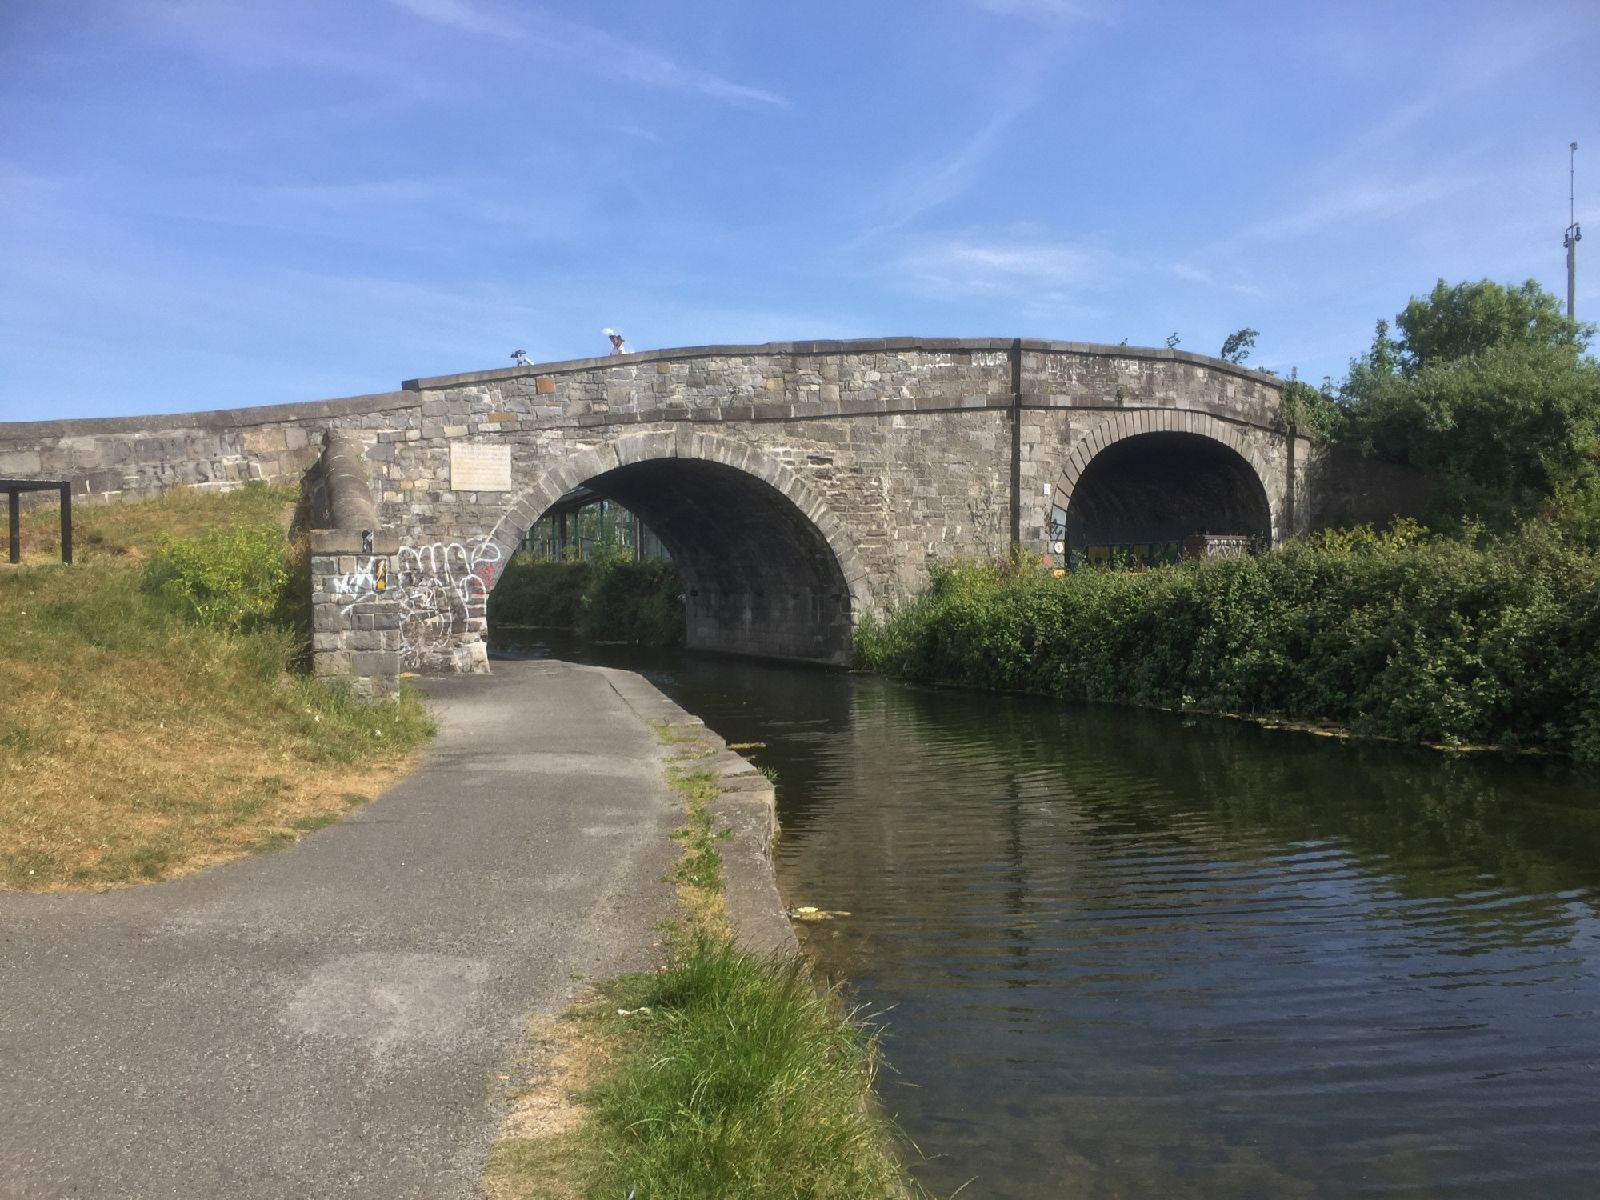
\includegraphics[width=\textwidth]{brppmbridge.jpg}
 	}
 	{
 		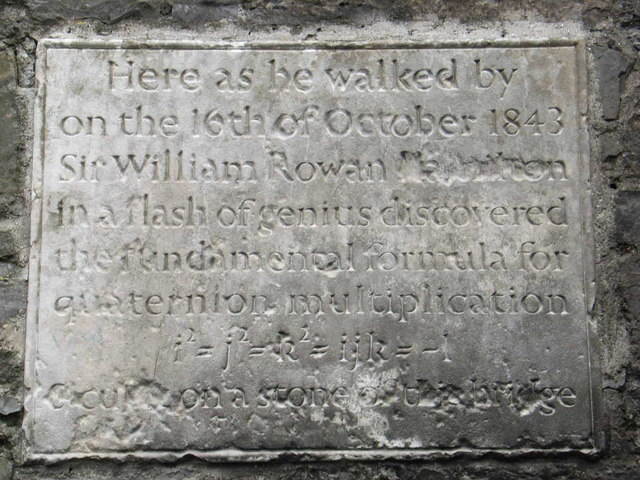
\includegraphics[width=\textwidth]{gamiltontable.jpg}
 	}
 	
    	Here as he walked by on the 16th of October 1843 Sir William Rowan Hamilton in a flash of genius discovered the fundamental formula for quaternion multiplication $i^2 = j^2 = k^2 = ijk = −1$ and cut it on a stone of this bridge.
 	
  		\hfill 	\hyperlink{frame:quaternion}{\beamerbutton{К лекции}}
 	
 \end{frame}
 
 
 
 
\begin{comment}
	
\end{comment}
 

\end{document}